\documentclass{article}
\usepackage{amsmath}
\usepackage{hyperref}
\usepackage{graphicx}
\newcommand{\tabincell}[2]{\begin{tabular}{@{}#1@{}}#2\end{tabular}}

\begin{document}
\begin{titlepage}
\title{EE 239AS \\Special Topics in Signals and Systems\\Project 2\\Classification Analysis\\Winter 2016} 
\author{Liqiang YU, Kaiming WANG and Jun FENG\\
904592975, 504592374, 304588434} 
\date{02-21-2016}
\end{titlepage}

\maketitle
\newpage
\tableofcontents
\newpage
\section{Introduction}
In this report, we implemented some classification models to classify the textual data from the "20 Newsgroups" dataset, including support vector machine (SVM), naive Bayes classifier and logistic regression classifier. Before the classification,there were some data preprocessing steps, like changing the number in each subset to make them balanced, transforming the textual data into TF-IDF matrix, implementing the singular value decomposition to reduce the dimension of TF-IDF matrix. The task included binary classification and multiclass classification. The results were measured with the metrics including the average of precision, recall and accuracy. Moreover, in order to characterize the trade-off between true positive rate (TPR) and false positive rate (FPR), the receiver operating characteristic (ROC) curve was plotted.\\
\\
The report is organized as follows: In section 2, we plot the numbers of ducument in 8 required classes. In section 3, we first employ TF.IDF to get term features, then we use a `TF-IDF like' stategery to get the most significant terms in 4 required classes.in section \ref{sec:binary} we discussed the classification results with support vector machine, naive Bayes classifier and logistics regression classifier. We compared the results from two SVM models : hard margin SVM and soft margin SVM, computed the precision, recall, accuracy and confusion matrix, plotted the ROC curve from three models. In section \ref{sec:multi}, we implemented two strategies for multiclass classification : "one VS one" and "one VS rest" and repeated the above procedures to test the results.
\section{Dataset and Problem Statement}
From the API documentation, we know that the 20 newsgroups dataset comprises around 18000 newsgroups posts on 20 topics split in two subsets: one for training (or development) and the other one for testing (or for performance evaluation). The split between the train and test set is based upon a messages posted before and after a specific date. \\
\\
The first thing is to have a look at datesets, and the most direct way is to get the number of documents per classes.The figure is shown in figure \ref{fig:problema}. We can find that since the number of document from 8 classes -comp.graphics,comp.os.ms-windows.misc,comp.sys.ibm.pc.hardware,comp.sys.mac.hardware are almost the same. The total number of documents in Computer technology is \emph{2343} while number of documents in Recreational activity is \emph{2389}. So when analyzing these 8 classes, it is unnecessary to adjust the number of documents when conducting any analysis within only 8 classes. \\
\\
However, if we want to make the datasets more balanced, we should import the data randomly, and reduce the number of 20 classes to the lowest number of original classes. We can just get first intended number of documents per class.
\begin{figure}[htbp]
\centering
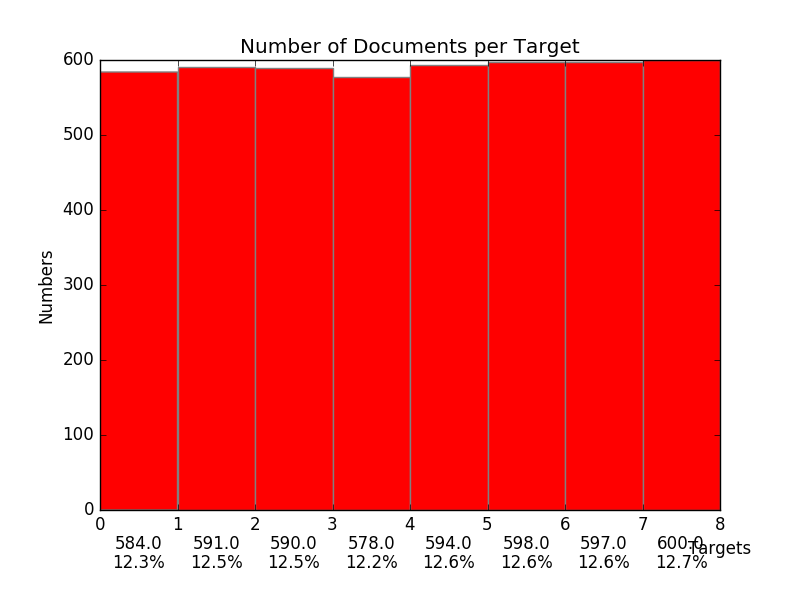
\includegraphics[width=.6\textwidth]{problema.png}
\caption{Numbers of Document per Target}
\label{fig:problema}
\end{figure}
\section{Modeling Text Data and Feature Extraction}
In this project, we will employ ``Big of Words'' assumption.The bag-of-words model is a simplifying representation used in natural language processing and information retrieval (IR). In this model, The text, or the document in our datasets, is represented as the bag (multiset) of its words, disregarding grammar and even word order. \\
\\
The bag-of-words model is commonly used in methods of document classification, where the (frequency of) occurrence of each word is used as a feature for training a classifier.However, before calculating the frequency of different terms, it is meaningful to remove different stems of verbs, stop words and punctuations.  By the way, we also remove special symbols and words containing numbers, since they are very rare.
\subsection{TFxIDF Vector Representations}
TF–IDF, which is the short for term frequency–inverse document frequency, is a numerical statistic that is intended to reflect how important a word is to a document in a collection or corpus.It is often used as a weighting factor in information retrieval and text mining. The tf-idf value increases proportionally to the number of times a word appears in the document, but is offset by the frequency of the word in the corpus, which helps to adjust for the fact that some words appear more frequently in general.\\
\\
We use TfidfVectorizer of sklearn to calculate the all \emph{11314} ducuments in 20 classes and finally we get \emph{54363} features.
\subsection{TFxICF and Significant Terms}
In this part, we would like to figure out whether a term is important to the class, so we can treat the whole set of documents in the same class as a ducument and calculate its TF.IDF, or so-called TF.ICF. However, we should pay attention that the defination of TF.ICF is one of common variation of IF.IDF, what is not used by the TfidfVectorizer of sklearn, we have to use CountVectorizer and try to achieve TF.ICF manually. Luckily, this procedure is quite easy. The result is in  Table \ref{10st}.
\begin{table}
\begin{center}
\caption{10 Most Significant Terms in 4 Classes }
\label{10st}
\begin{tabular}{|l||l|l|l|l|}
\hline
Rank & \tabincell{c}{comp.sys.ibm.\\pc.hardware} & \tabincell{c}{comp.sys.\\mac.hardware} & misc.forsale & soc.religion.christian \\
\hline
1& penev & powerbook & sabretoo & clh\\
2& balog & lcii & liefeld & liturgy\\
3& scsiha & iis & hobgoblin & kulikauska\\
4& husak & adb & uccxkvb & mmalt\\
5& laton & bmug & radley & copt\\
6& fasst & iivx & kou & caralv\\
7& buslog & iifx & keown & monophysit\\
8& korenek & jartsu & koutd & mussack\\
9& mbyet & firstclass & spiderm & sspx\\
10& dric & macus & mcfarlane & atterlep\\
\hline 	
\end{tabular}
\end{center}
\end{table}
\section{Binary Classification}\label{sec:binary}
In the binary classification problem, we chose eight classes and wanted to seperate them into two classes : Computer Technology and Recreational Activity. We assign the tag 0 to Computer Technology subclasses and tag 1 to Recreational Activity subclasses. The number of each subclass is almost the same so there is no need to balance them.
\subsection{Hard Margin SVM}
In the hard margin SVM, the objective function is
\begin{equation*}
min \frac{1}{2}\Vert W \Vert _2 ^2
\end{equation*}
And the constraints is
\begin{equation*}
y_i(W^T\overrightarrow{x_i}+b)\geq 1, i\in\lbrace 1, ..., n \rbrace
\end{equation*}
\\
In the program, we set C to 100000 to simulate the effect of hard margin (the tutorial said it's zero but I think it's wrong and I have talked about it with the TA). The average precision is 96.61\%, the average recall is 98.49\% and the accuracy is 97.49\%.The confusion table is shown in Table \ref{tb:confu}. The ROC curve  is shown in figure \ref{fig:roc_hard}
\begin{table}
\begin{center}
\caption{The confusion matrix of hard margin SVM}
\label{tb:confu}
\begin{tabular}{|c|c|c|}
\hline
& Predicted Comp& Predicted Rect\\
\hline
Actual Comp&1505&55\\
\hline
Actual Rect&24&1566\\
\hline 	
\end{tabular}
\end{center}
\end{table}

\begin{figure}[htbp]
\centering
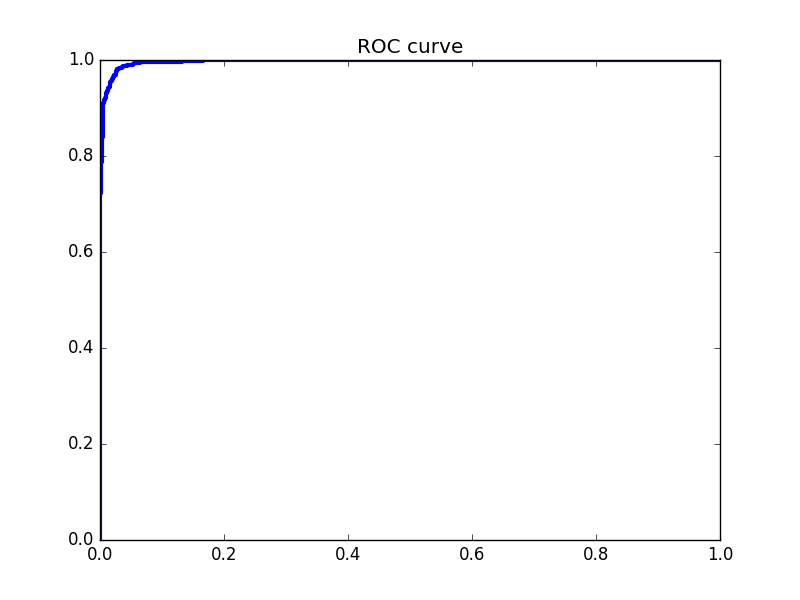
\includegraphics[width=.6\textwidth]{roc_hard.png}
\caption{The ROC curve for hard margin SVM}
\label{fig:roc_hard}
\end{figure}
\subsection{Soft Margin SVM}
The problem of the hard margin model is that it may overfit the data, therefore it's better to use the soft margin SVM. In the soft margin model, we add error parameter in the objective function and the constraints. Thus the objective function is changed to the following:
\begin{equation*}
min \frac{1}{2}\Vert W \Vert _2 ^2 + \gamma\sum_{i=1}^{n}\xi _i
\end{equation*}
\\
Accordingly, the constraints are changed to the following:
\begin{equation*}
y_i(W^T\overrightarrow{x_i}+b)\geq 1-\xi _i,  \xi _i \geq0,  i\in\lbrace 1, ..., n \rbrace
\end{equation*}
\\
The $\gamma$ is the hyperparameter here and different $\gamma$ will affect the classification results. We implemented 5-fold cross validation to fit the model and choose the $\gamma$.  The best $\gamma$ we can get is 1000. The average precision is 96.61\%, the average recall is 97.96\% and the accuracy is 97.27\%. The confusion matrix is shown in Table\ref{tb:confu_soft}. The roc curve is shown in figure \ref{fig:roc_soft}.
\begin{table}
\begin{center}
\caption{The confusion matrix of soft margin SVM with $\gamma$ = 100000}
\label{tb:confu_soft}
\begin{tabular}{|c|c|c|}
\hline
& Predicted Comp& Predicted Rect\\
\hline
Actual Comp&764&27\\
\hline
Actual Rect&16&769\\
\hline 	
\end{tabular}
\end{center}
\end{table}

\begin{figure}[htbp]
\centering
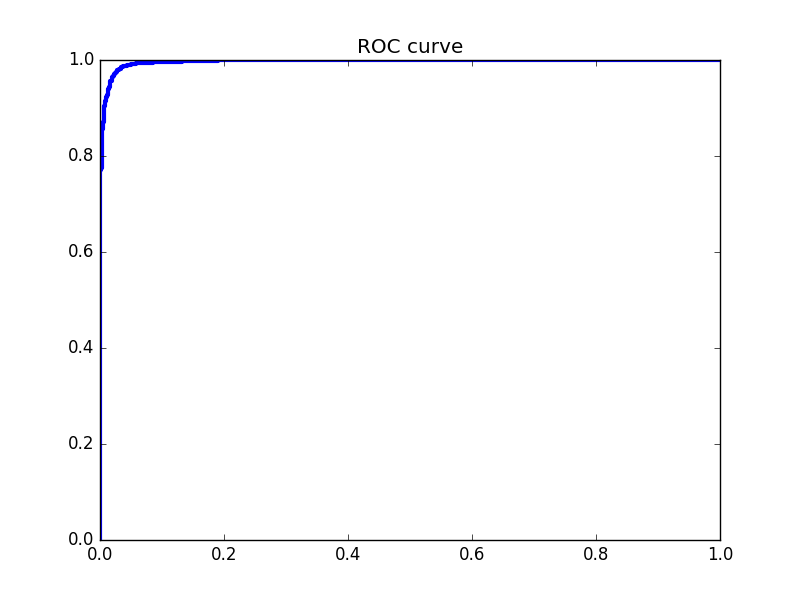
\includegraphics[width=.6\textwidth]{roc_soft.png}
\caption{The ROC curve for soft margin SVM}
\label{fig:roc_soft}
\end{figure}
\section{Multiclass Classification}\label{sec:multi}
\section{Conclusion}
In this project, we aimed to finish some classification tasks with the textual data provided by the "20 Newsgroup" dataset. We classified 8 subclasses into 2 classes with the hard margin SVM, soft margin SVM, naive Bayes classifier and logistics regression classifier. The comprehensive results is shown in the Table \ref{tb:binaryresults}. As for the multiclass classification, the comprehensive results is shown in Table \ref{tb:multiresults}.
\begin{table}
\begin{center}
\caption{The comprehensive results of binary classification}
\label{tb:binaryresults}
\begin{tabular}{|c|c|c|c|}
\hline
& Accuracy& Precision& Recall\\
\hline
hard margin SVM& 97.49\%&96.61\% &98.49\% \\
\hline
soft margin SVM& 97.27\%&96.61\% &97.96\% \\
\hline 	
Bayes& & & \\
\hline
Logistic Regression& & &\\
\hline
\end{tabular}
\end{center}
\end{table}

\begin{table}
\begin{center}
\caption{The comprehensive results of multiclass classification}
\label{tb:multiresults}
\begin{tabular}{|c|c|c|c|}
\hline
& Accuracy& Precision& Recall\\
\hline
SVM& \%&\% &\% \\
\hline
Bayes& & & \\
\hline
Logistic Regression& & &\\
\hline
\end{tabular}
\end{center}
\end{table}
\end{document}